\documentclass[11pt,a4paper,fleqn]{article}
\usepackage{geometry}
\geometry{margin={0.3in,0.3in}}

\usepackage{mathtools}

\mathtoolsset{
  showonlyrefs,
}

\usepackage{tikz} %tikz is used to draw the glyphs
\usetikzlibrary{arrows,scopes} %tikz libraries used to draw the glyphs

\usepackage[%
bookmarksopen=true,
colorlinks=true
]{hyperref}

\usepackage{tcolorbox}
\tcbuselibrary{theorems}

\tcbset{
boxrule=0.8pt,
arc=1px,
parbox=false, %?
halign=left,halign upper=left,halign lower=left,
coltitle=black,
colbacktitle=white,
colback=white}

\NewTcbTheorem[no counter, list inside=facts]%
{fact}{Fact}%
{fonttitle=\bfseries,attach title to upper={\par}}{fact}
\newtcolorbox{exec}{}

\setlength\parindent{0pt}
\setlength{\parskip}{0.6\baselineskip}
\numberwithin{equation}{section}

\usepackage{nopageno}
\usepackage{tocbibind}
\usepackage[none]{hyphenat}

\usepackage{xcolor}

\usepackage{unicode-math}
\setmathfont{texgyrepagella-math.otf}

% MY ===
\newcommand{\go}{$ \rightarrow\ $}
\newcommand{\TODO}{{\color{red}{\fbox{TODO}}\ }}
\newcommand{\Concept}{\textbf}

% Notations ===

\def\bm{\ensuremath{\symbf}}

% STD symbols ===
\newcommand{\Del}{\ensuremath{\nabla}}
\newcommand{\UnitVec}[1]{\ensuremath{\bm{\hat{#1}}}} % unit vector
\newcommand{\D}{\ensuremath{\,d}}

\newcommand{\ScriptRMag}{
  \resizebox{!}{1.25ex}{
    \begin{tikzpicture}[>=round cap]
      \clip (0.09em,-0.05ex) rectangle (0.61em,0.81ex);
      \draw [line width=.11ex, <->, rounded corners=0.13ex] (0.1em,0.1ex) .. controls (0.24em,0.4ex) .. (0.35em,0.8ex) .. controls (0.29em,0.725ex) .. (0.25em,0.6ex) .. controls (0.7em,0.8ex) and (0.08em,-0.4ex) .. (0.55em,0.25ex);
    \end{tikzpicture}
  }
}

\newcommand{\ScriptR}{
  \resizebox{!}{1.3ex}{
    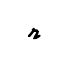
\begin{tikzpicture}[>=round cap]
      \clip (0.085em,-0.1ex) rectangle (0.61em,0.875ex);
      \draw [line width=.2ex, <->, rounded corners=0.13ex] (0.1em,0.1ex) .. controls (0.24em,0.4ex) .. (0.35em,0.8ex) .. controls (0.29em,0.725ex) .. (0.25em,0.6ex) .. controls (0.7em,0.8ex) and (0.08em,-0.4ex) .. (0.55em,0.25ex);
    \end{tikzpicture}
  }
}

\begin{document}

\section{Notations}

Griffiths' Script R, its magnitude and related unit vector are defined as
\begin{align}
  \ScriptR &= \bm{r} - \bm{r'} \\
  \ScriptRMag &= |\bm{r} - \bm{r'}| \\
  \hat{\ScriptR} & = \frac{\ScriptR}{\ScriptRMag} = \frac{\bm{r} - \bm{r'}}{|\bm{r} - \bm{r'}|}
\end{align}
where $\bm{r}$ is a field point and $\bm{r'}$ is a the source point.


\section{Vector Analysis}
\subsection{The del operator}

The Del operator $\Del$ is defined as
\begin{equation}
  \newcommand{\utp}[1]{\UnitVec{#1}\frac{\partial}{\partial #1}}
  \Del =\utp{x} + \utp{y} + \utp{z}
\end{equation}
where \UnitVec{x},\UnitVec{y},\UnitVec{z} are unit vectors.

The $\Del$ is an vector operator than acts upon vectors.

For example, $\Del$ can act via

\begin{itemize}
  \item Scalar function \go $\Del T$ (Gradient)
  \item Dot product \go $\Del\cdot\vec{v}$ (Divergence)
  \item Cross product \go $\Del \times \vec{v}$ (Curl).
\end{itemize}


\section{Diary}

\subsection{Euler's homogeneous function}

\begin{fact}{Define homogeneous function}{}
  Let $f$ be a function of n variables defined on a set $S$ for which $(tx_1,...,tx_n)\in S$ whenever $t>0$ and $(x_1,...,x_n)\in S$, and let $k$ be a number.

  Then $f$ is homogeneous of degree k if $f(tx_1,...,tx_n) = t^k f(x_1,...,x_n)$.
\end{fact}

Its partial differential can be written in many forms:

\begin{align}
  k f(x_1,...,x_n)
  & = \sum_{i=1}^{n} x_i \left(\frac{\partial f(x_i)}{\partial a_i} \right) \\
  & = \sum_{i=1}^{n} x_i f_i'(x_1,...,x_n) \\
  & = x\cdot\Del f(x).
\end{align}

This models multi-component systems where certain observable property changes proportionally to each components' rate of change.

\subsubsection{Application on ideal gas}
Assume some ideal gas system has fixed temperature $T$ and pressure $P$, then the system's volume $V_{system}$ will depends on the components' molal numbers $n_i$ and volume $V_i$ of the system. This can be written as
\begin{equation}
  V_{system} = \sum n_i \left( \frac{\partial V_i}{\partial n_i} \right)_{T,P,{n_j|j\neq i}}.
\end{equation}

The $\left( \cdotp \right)_{T,P,{n_j|j\neq i}}$ denotes fixed part of the system \go temperature, pressure and other components.

Then we can abstract the concept of \Concept{Partial molal volume} of component $i$ which is $\overline{V_i} = \left( \frac{\partial V_i}{\partial n_i} \right)_{T,P,{n_j|j\neq i}}$.
\begin{equation}
  V_{system} =\sum n_i \overline{V_i}
\end{equation}

The $\overline{V_i}$ means the amount of volume that will increase when adding infinitesimal amount of component $i$ to the system at constant temperature and pressure while keeping other components at fixed number will increase.

This method of abstracting can be generalized into \Concept{Partial molar quantities} or \Concept{Partial molal properties}.

\subsection{Legendre Transformation}

Basically, for a function $f(x,y)$, a equation like
\begin{equation}
  \D f = \frac{\partial f}{\partial x} x + \frac{\partial f}{\partial y} y= p \D x + q \D y
\end{equation} can be transformed into
\begin{align}
  g &= f - qy = f - \frac{\partial f}{\partial y}y\\
 \D g &= p \D x - y \D q.
\end{align}

Alternatively, the transformation can be written as
\begin{equation}
  G(X) = F(x) - \frac{\partial F(x)}{\partial x} x.
\end{equation}

Note that
\begin{align}
  \frac{\partial g}{\partial x} &= p =  \partial f / \partial x \\
  \frac{\partial g}{\partial q} &= -y.
\end{align}
Also note that
\begin{align}
  \frac{\partial^2 g}{\partial q\partial x} &= \frac{\partial}{\partial q} \frac{\partial g}{\partial x} = \left(\frac{\partial p}{\partial x}\right)_x \\
  \frac{\partial^2 g}{\partial x \partial q} &= \frac{\partial}{\partial x} \frac{\partial g}{\partial q}= \left(- \frac{\partial y}{\partial x}\right)_q.
\end{align}
Assuming $\frac{\partial^2 g}{\partial q\partial x} = \frac{\partial^2 g}{\partial x \partial q}$, then we get
\begin{equation}
  \left(\frac{\partial p}{\partial x}\right)_x =  \left(- \frac{\partial y}{\partial x}\right)_q.
\end{equation}
\begin{fact}{Rediscover of Legendre transformation}{}
  Given function $f(x,y)$ and its derivative
  \begin{equation}
    \D f=\frac{\partial f}{\partial x}\D x + \frac{\partial f}{\partial y}\D y.
  \end{equation}
  Let $\partial f / \partial x = p$ and $\partial f / \partial y = q$, then
  \begin{equation}
    \D f = p \D x + q \D y.
  \end{equation}
  Subtract from $\D f$ the quantity $\D (qy)$, then
  \begin{align}
    \D f - \D (qy) &= p \D x + q \D y - d(qy) = p \D x + q \D y - q \D y - y \D q \\
    \D (f-qy) &= p \D x - y \D q.
  \end{align}
  Then let's define $g = f-qy = f - \frac{\partial f}{\partial y} y$ which has derivative
  \begin{equation}
     \D g = \D (f-qy) = p \D x - y \D q.
  \end{equation}
\end{fact}

\begin{exec}
  Transform $\D u = T \D s  - p \D v$ to  $f(T,v)$.
  \tcblower
  \begin{align}
        f&=u-Ts\\
    \D f &= -p \D v - s \D t
  \end{align}
\end{exec}

\end{document}
